\chapter{Практическая часть. Исследование тематического профиля Интернет-СМИ Омской области} \label{chapt2}
\section{Определение целей исследования} \label{sect2_1}
В данной части работы мы разработаем и проведём небольшое исследование, цель которого состоит в построении тематического профиля Интернет-СМИ Омской области. На примере данного исследования будут показаны возможности метода интеллектуального анализа текста в социологии и дано представление о том, как конкретно и с использованием каких инструментов пройти все ранее выделенные этапы интеллектуального анализа текста. Исследование тематического профиля будет включать в себя следующие задачи:

\begin{enumerate}
\item Оценка доступности и характера данных. Сбор данных.
\item Выявление распределения статей и комментариев в времени.
\item Предварительная обработка данных.
\item Тематическое моделирование
	\begin{enumerate}
	\item Определение оптимального количества тем.
	\item Создание модели LDA
	\item Выявление распределения статей по темам
	\end{enumerate}
\item Анализ комментариев
	\begin{enumerate}
	\item Выявление распределения комментариев в времени
	\item Определение тональности комментариев
	\item Определение тональности по темам
	\end{enumerate}

\end{enumerate}
\todo[inline]{Задачи надо формулировать более крупно? Суть работы в том, чтобы выделить темы и определить отношение комментаторов к этим темам. Две задачи}

\section{Оценка доступности и характера данных. Сбор данных.} \label{sect2_2}
Прежде чем начать сбор данных, нам придётся поставить перед собой несколько вопросов, представляющих особенную трудность в данного типа исследованиях. А именно, необходимо определить, что будет являться носителем знаний по исследуемой проблеме (т. е. эмпирическим объектом исследования), каковы границы генеральной совокупности, какой метод будет являться адекватным для построения выборочной совокупности, как определить качественные и количественные характеристики выборки, каковы критерии репрезентативности выборки \cite{methodlogy_internet}.

\textbf{Определение эмпирического объекта.} 

В исследованиях подобного вида эмпирическим объектом могут быть посты, комментарии, отдельные высказывания и многое другое. В нашем случае можно сказать, что источником знаний о проблемах, затронутых в данном исследовании являются новостные статьи в Интернет-СМИ Омской области. Углубляясь дальше, мы должны решить какие аспекты статей нас интересуют. Статья в Интернет-СМИ -- не просто текст. Это документ, который имеет свою структуру. В этой структуре нас буду интересовать такие элементы как собственно текст, название, дата публикации, комментарии к статье, принадлежность к тому или иному СМИ. Первая причина, по которой они были выбраны состоит в представленности этих элементов в статьях каждого из рассматриваемых нами Интернет-СМИ. Количество просмотров и ключевые слова (тэги), например, на некоторых ресурсах бывают не указаны. Другая причина -- достаточность данных элементов для решения исследовательских задач.

\textbf{Определение генеральной и выборочной совокупностей.}

Определение эмпирического объекта позволяет перейти к установлению генеральной и выборочной совокупностей. На сегодняшний день не существует единой позиции как определять эти совокупности при исследование текстов в сети Интернет. Каждый исследователь придумывает сам, каким способом наиболее полно реализовать принципы выборки.

Зизи Папачарисси \cite{zizi}, например, при исследовании блогосферы в качестве генеральной совокупности определяла все блоги, расположенные на платформе blogger.com. Она объясняет свой выбор тем, что это наиболее популярный и большой по числу блоггеров англоязычный сайт, который предоставляет возможности для персональных публикаций в стиле любительской журналистики. Любой блог, по мнению Папачарисси, размещённый это этом сайте, представлял собой единицу анализа, отвечающую по своим характеристикам признакам принадлежности к генеральной совокупности. Однако нельзя согласиться, что блоги с blogger.com репрезентативны относительно всей блогосферы. Выборочную совокупность блогов Папачарисии составляла использую случайную отправную точку и случайный выборочный интервал. Однако исследователем не было оговорено, какие именно данные вводились в поисковую систему для поиска релевантных блогов и какие именно блоги считались релевантными, сколько блогов входило в генеральную совокупность и почему было отобрано именно 260. К тому же использование поисковых систем для поиска блогов выглядит сомнительно: алгоритмы данных систем неизвестны исследователю и нельзя сказать, почему были отобраны эти блоги, а не иные.

Генеральную совокупность в данном исследовании составляют новостные статьи Интернет-СМИ г. Омска. Омским Интернет-СМИ считается веб-сайт, ставящий своей задачей выполнение функции средства массовой информации (СМИ) в сети Интернет и ориентированный на аудиторию, живущую в Омской области. По данным Агентства Региональных Исследований за июнь 2014 года в Омске работает около 18 Интернет-СМИ с месячным количеством уникальных посетителе в месяц более 10000 \cite{ari_rating}. 

Использование данных со всех возможных ресурсов -- очень трудоёмкая задача, поскольку добавление нового источника требует практически полного переписывания соответствующей части компьютерной программы, ответственной за собственной сбор данных, и частичной переработки модуля предварительной обработки. Вполне привычным для социолога решением будет конструирование выборки. Однако как рассчитать выборку, если не известны объёмы генеральной совокупности? А даже если бы мы знали количество статей каждого из рассматриваемых Интернет-СМИ за любой промежуток времени, разве было бы корректно использовать традиционные методы определения выборочной совокупности в такого типа исследованиях? Эта аналогия видится некорректной по причине кардинального различия эмпирических объектов -- человека и текста. При определении людей в качестве эмпирических объектов исследования социолог как правило предполагает, что они в равной степени могут служить источником информации о проблеме. Исключение из этого правила встречается, когда исследователь дополнительно изучает мнение экспертов. Но такие опросы -- это отдельная часть исследования, в которой как правило используются другие методы сбора и анализа информации.

Тексты в Интернете не равнозначны по своему значению. По нашему мнению, новостная статья заслуживает тем больше внимания, чем больше количество её просмотров. Статья, которую никто не прочитал, -- не существует в медийной сфере. %Но не все Интернет-СМИ предоставляют эту информацию, поэтому можно опереться на косвенный индикатор -- количество просмотров всех статей исследуемого ресурса. То есть мы предполагаем, что чем больше совокупное количество просмотров у одного ресурса, тем более сильно влияние каждой его отдельной статьи.

В нашем случае необходимо определить несколько Интернет-СМИ, все статьи которых будут отобраны для исследования. Мы решили, что при определении значимости статьи определяющей характеристикой является количество просмотров. Хотя Интернет-СМИ в Омске и немало, не все из них одинаково популярны. Судя по тем же данным АРИ \cite{ari_rating}, в Омске существует всего четыре новостных ресурса, страницы которых просматривают более одного миллиона раз в месяц. На их долю приходится 65\% всех просмотров. Представляется, что анализ статей, получивших более половины всех просмотров является достаточным основанием для выделения их в качестве выборочной совокупности, по результатом анализа которой можно будет делать выводы об омских Интернет-СМИ в целом. Таким образом в исследовании будут проанализированы все новостные статьи с сайтов <<Город 55>>\footnote{\href{http://gorod55.ru}{http://gorod55.ru}}, <<БК55>>\footnote{\href{http://bk55.ru}{http://bk55.ru}}, <<НГС Омск>>\footnote{\href{http://ngs55.ru}{http://ngs55.ru}}, <<Омск-Информ>>\footnote{\href{http://omskinform.ru}{http://omskinform.ru}} за период с 1 сентября 2013 по 1 сентября 2014. Новостными статьями будут считаться те, которые публикуются на данном ресурсе в разделе <<Новости>>. Статьи из категорий <<Работа>>, <<Объявления>>, <<Блоги>> и др. в анализе не участвуют.

Определившись с данными, которые необходимо собрать, нужно решить, каким способом это сделать, т. е. с использованием каких инструментов и технологий будет производится сбор данных. Для этого мы будем использовать язык программирования Python. Основанием для такого выбора является его простота, поддержка многопоточности, что полезно для более быстрого сбора данных, наличие сторонних библиотек, что позволяет избежать написание рутинного кода, а также то, что обработка и анализ данных также будет производится на этом языке -- это обеспечивает некоторую консистентность исследования. %Ближайшей альтернативой данному решению нам видится использование программной платфоры node.js из-за хорошей поддержки асинхронных запросов (и, следовательно, высокой скорости) и наличия множества качественных библиотек для сбора данных или языка R, который традиционно популярен в академической среде для сбора и анализа данных.

%Для хранения данных будет использована база данных MongoDB. Как говорилось выше, в БД будут присутствовать следующие поля: называние статьи, содержимое статьи, ссылка на статью, дата публикации, количество комментариев и список комментариев к статье. Статьи с каждого источника будут храниться в отдельной коллекции.

Результаты сбора данных следующие:
\begin{itemize}
\item C сайта gorod55.ru было собрано 6302 статьи
\item Больше всего новостных статей за указанный промежуток времени было опубликовано на bk55.ru -- 14078 статей  на bk55.ru
\item Наименьшее количество статей -- 4780 -- было найдено на ngs55.ru
\item 8727 статей по указанным параметрам было собрано с сайта omskinform.ru
\end{itemize}

Всего, таким образом, в анализе участвовало 33887 статей.

На этом этапе крайне важно контролировать корректность и полноту собираемых данных. Сложнее всего было с сайтом bk55.ru, поскольку в нём использовались несколько различных шаблонов для отображения информации, каждый из которых необходимо было отследить и создать под него набор правил для извлечения данных.

Исследуем распределение статей во времени, построив график (рисунок \ref{fig:docs_by_day}), на оси $x$ которого отложены дни, а на оси $y$ -- количество статей, опубликованных в каждый из дней. Дополнительно выделим выходные дни красным цветом.

\begin{figure}
	\centering
    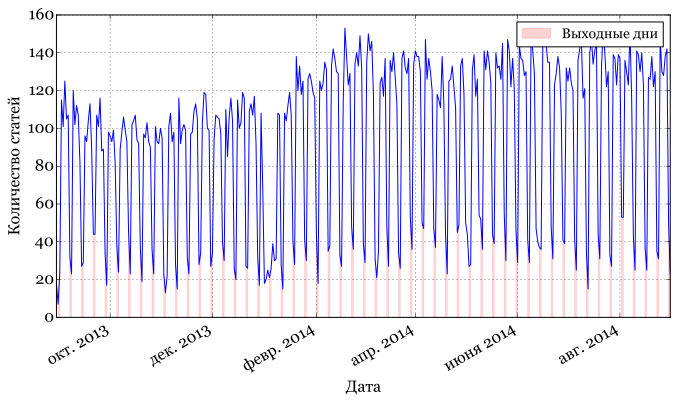
\includegraphics[totalheight=10cm]{docs_by_day}
    \caption{Количество статей по дням}
    \label{fig:docs_by_day}
\end{figure}

Анализ графика позволяет сделать несколько выводов. Во-первых, заметна неравномерность распределения статей по дням недели. В будние дни в среднем публикуется статей 116, в то время как в выходные -- только 33. Во-вторых, наблюдается сильное снижение количества публикаций на новогодние каникулы. Наблюдаемые колебания очевидно зависят от рабочего графика сотрудников СМИ.

\section{Предварительная обработка данных}

Предварительная обработка данных -- один из важнейших этапов в анализе текста. Наша цель на этом этапе -- удаление несущественных и вносящих помехи данных и преобразование данных к удобному для анализа виду.

На самом деле удалять несущественные данные мы начали ещё на этапе сбора данных, поскольку перед записью в базу данных весь текст, если это было необходимо, очищался от HTML-разметки. Преобразование же данных на том этапе заключалось в конвертации текста, содержащего информацию о дате публикации, в специальный тип данных, позволяющий обращаться к этим данным как к дате, например, производить выборку статей за определённый период.

Дальнейшая обработка данный заключалась в следующем:

\begin{enumerate}
\item Удаление лишней информации
\item Перевод текста в нижний регистр
\item Токенизация
\item Удаление пунктуации
\item Лемматизация
\item Удаление стоп-слов
%\item Замена слов
\end{enumerate}
Поясним некоторые из этих этапов.

\subsubsection{Удаление специфических признаков}
Данный этап предварительной обработки данных заключается в удалении из каждой статьи признаков, свидетельствующих о её принадлежности к какому-либо источнику. Если посмотреть на полученные тексты, то можно увидеть, что редакция каждого СМИ устанавливает собственные правила оформления документов, касающиеся оформления ссылок на источники данных, фотографий, указание имён авторов. В случаем если эти отличительные черты не будут устранены, алгоритмы тематического моделирования, которые мы в дальнейшем собираемся применить к собранному корпусу текстов, будут стремиться образовать темы вокруг источников. Процедура унификации статей из различный источников достаточно трудоёмка и требует ручного анализа множества статей с каждого из них, с тем чтобы выявить в них специфические черты для каждого сайта. Такими чертам могут быть имена журналистов данного издания или правила оформления фото и видео материалов (например, около каждой фотографии может указываться копирайт).

Например, чтобы удалить имена журналистов из текстов статей на сайте bk55.ru, необходимо было во-первых, составить их список. Для составления списка, была написана небольшая программа, выводящая два последних слова каждого документа, если они начинались с заглавной буквы (как правило имена авторов указывались в конце документа, хоть и не всегда). Из полученного списка примерно в пятьсот пар были вручную отсеяны пары, не являющиеся именем и фамилией. Те пары из этого списка, которые встречались больше двух раз, считались нами именем и фамилией журналистов сайта bk55.ru. На последнем этапе фамилии журналистов удалялись из каждого документа. К тому же, так как после имён журналистов часто указывалась другая мета-информация (главным образом ссылки источники информации), то также удалялся весь текст после имён, если по размеру этот текст не превышал определённое количество символов (чтобы предотвратить удаление не мета-информации). 

После устранения специфической информации данные из различных источников объединялись в единый корпус и подвергались дальнейшей обработке.

\subsubsection{Токенизация}
Следующим этапом предварительной обработки текста является токенизация. Именно с неё начинается обработка естественного языка как наука и как конкретная деятельность \cite{Webster1992}. Под токенизацией понимают процесс сегментации текста на отдельные части, называемые токенами. Именно токены являются теми первичными элементами, которые непосредственно участвуют в процессе анализа. 

Выделяют два основных признака токена -- лингвистическая значимость и методологическая полезность \cite[стр. 1106]{Webster1992}. В языках с иероглифической письменностью токенизация является серьёзной проблемой, поскольку один иероглиф может обозначать как морфемы (в таком случае он не удовлетворяет требованиям для того, чтобы считаться токеном), так и целые слова. В английском и русском языках проблема токенизации не стоит так остро и чаще всего токены определяются через пробелы между словами и знаки препинания. Тем не менее, даже в этих языках существуют определённые нюансы.

Нами было протестировано несколько алгоритмов токенизации (токенайзеры TreebankWordTokenizer, WordPunctTokenizer, PunctWordTokenizer и WhitespaceTokenizer из программы NLTK\footnote{\href{http://www.nltk.org}{http://www.nltk.org}} и токенайзер из Pattern\footnote{\href{http://www.clips.ua.ac.be/pattern}{http://www.clips.ua.ac.be/pattern}}). Корректнее всех выделял токены изначально не презназначенный для работы с русски языком токенайзер из программы Pattern. Например, он единственный интерпретировал URL'ы как цельные токены, не выделяя в них отдельные сегменты на основе знаков препинания.

\subsubsection{Стемминг и лемматизация}
После токенизации и удаления токенов, являющихся знаками препинания, мы перешли от представления документов как набора символов к документам как списку слов. Дальнейшие наши шаги будут направлены на уменьшение длинны этого списка, т. е. на снижение как общего количества токенов, так и количества их уникальных единиц. Необходимость этих шагов обусловлена желанием снизить вычислительную сложность анализа данных.

Первый шаг направлен на снижение количества уникальных токенов. Для компьютера различные формы одного и того же слова являются совершенно разными словами. Существует два способа для приведения словоформ к одной лексеме. Первый, самый простой, называется стемминг. Он состоит в отсечении слово- и формообразующих частей -- префиксов, суффиксов, окончаний, в результате чего остаётся основа слова -- неизменная часть, выражающая его лексическое значение.

Более сложным подходом к решению проблемы унификации словоформ является лемматизация. Лемматизация -- это процесс приведения словоформы к лемме — её нормальной (словарной) форме. В русском языке нормальная форма имени существительного имеет именительный падеж и единственной число, для прилагательных добавляется требование мужского рода, а глаголы, деепричастия и причастия в нормальной форме должны стоять в инфинитиве.

Для постановки слова в нормальную форму необходимо иметь словарь, где для каждого слова определены его характеристики, т. е. часть речи, падеж, число, род, форма глагола (если это глагол). Создание такого словаря требует колоссальных трудов. В отличии от этого, стемминг предполагает наличие лишь списка приставок, суффиксов и окончаний, количество которых исчисляется несколькими десятками. К счастью, для русского языка существует так необходимый для лемматизации словарь, созданный в рамках проекта OpenCorpora\footnote{\href{http://opencorpora.org}{http://opencorpora.org}}. Использующая этот словарь программа pymorphy2\footnote{\href{https://pymorphy2.readthedocs.org}{https://pymorphy2.readthedocs.org}} позволяет приводить слова к нормальной форме.

Между вышеозначенными способами мы выбрали лемматизацию, поскольку получаемые в результате этого процесса леммы удобнее интерпретировать, по сравнению с усечёнными основами слов, значение которых не всегда легко восстановить.

\subsubsection{Удаление стоп-слов}
Дальнейшие усилия по уменьшению количества токенов связаны с удалением так называемых стоп-слов. Эти слова, сами по себе почти не неся полезного смысла, тем не менее, необходимы для нормального восприятия текста. Чаще всего к разряду стоп-слов относятся служебные части речи -- предлоги, союзы, частицы. Будучи широко распространёнными в тексте, они мало могут сказать о его теме.

В качестве базы для списка стоп-слов был использован список русских стоп-слов из программы NLTK. Однако его нельзя считать достаточно полным. Включая в себя 151 слово, данный список покрывает лишь самые основные случаи. Для его пополнения необходимо обратиться к собранным ранее данным. На их основе был составлен список наиболее часто встречающихся в корпусе токенов. Среди них были выбраны несколько десятков слов, наиболее точно подходящие под описание стоп-слов (это, который, такой, некоторый, другой, тот и др.), которые затем были добавлены в соответствующий список. Представляется, что такой список, дополненный словами, выбранными из числа наиболее распространённых, является достаточно полным, поскольку стоп-слова по своему характеру всегда относятся к наиболее часто встречающимся в тексте. Редкие слова как правило свидетельствуют о принадлежности текста к какой-либо теме, а потому не могут относиться к разряду стоп-слов.

%\subsubsection{Замена слов}
%В заключение, для удобства анализа была произведена замена некоторых слов. Данная замена включала в себя во-первых, раскрытие аббревиатур (рф $\to$ россия, ул $\to$ улица и др.), а во-вторых, лемматизацию токенов, которые не были лемматизированы автоматически (расина $\to$ расин, парка $\to$ парк). Данный шаг не является обязательным и может быть без последствий пропущен.

\subsubsection{Выводы}
Как видно, в общих чертах данный набор процедур повторяет составляющие предварительной обработки данных из методологии CRISP-DM.

Необходимо отметить, что после каждой операции с данными на этапе предварительной обработки следует контролировать последствия производимых изменений. Такой контроль поможет выявить проблемы на раннем этапе, что убережёт от лишней работы в будущем \footnote{Например, одной из таких проблем, выявленных на раннем этапе, было наличие в текстах некоторых СМИ неразрывных пробелов. Они мешали токенизации, поскольку сегментация производилась по обычным пробелам. Так как визуально неразрывные пробелы почти ничем не отличаясь от обычных, их наличие было установлено только благодаря ручному контролю результатов токенизации. Решением стала замена всех неразрывных пробелов на обычные.}.

\section{Тематическое моделирование}

\subsection{Обзор методов тематического моделирования}
% обзор методов
% история
% задачи
% LDA
% применение LDA
Одна из главных задач данного исследования -- выявление тем собранных ранее статей. Данная задача известна как тематическое моделирование (topic modeling).

Построение тематическое модели может рассматриваться как задача одновременной кластеризации документов и слов по одному и тому же множеству кластеров, называемых темами. В терминах кластерного анализа тема -- это результат би-кластеризации, то есть одновременно кластеризации и слов и документов по их семантической близости. Обычно выполняется нечёткая кластеризация, то есть документ может принадлежать нескольким темам в различной степени. Таким образом, сжатое семантическое описание слова или документа представляет собой вероятностное распределение на множестве тем. Процесс нахождения этих распределений и называется тематическим моделированием \cite{korshunov2012}.

Тематическое моделирование активно развивается последние двенадцать лет и находит своё применение в широком спектре приложений. Оно применяется для выявления трендов в научных публикациях, для классификации и кластеризации документов, изображений и видеопотоков, для информационного поиска, в том числе многоязычного, для тегирования веб-страниц, для обнаружения текстового спама, для рекомендательных систем и других приложений \cite[стр. 4]{voroncov2013}. 

Тематическое моделирование постепенно находит признание и среди социологов. Помимо уже упоминавшегося исследования египетских СМИ \cite{EgyptianUprising2012}, можно упомянуть проект, цель которого заключалась в отслеживании того, как менялось освещение СМИ культурной политики США \cite{poetics_topics}.

В российской социологии подобного вида исследования проводились исследовательским коллективом Лаборатории Интернет-исследований Санкт-Петербургского филиала ВШЭ \cite{kolcovalda}. Материалом для тематического моделирования послужили записи 2000 самых популярных блогеров по рейтингу популярности Живого Журнала. Для тематического моделирования в данном исследования была использована созданная в лаборатории программа TopicMiner, которая сменила использовавшийся ранее Stanford Topic Modeling Toolbox. Обе этих программы реализовывают алгоритм латентного размещения Дирихле с сэмплированием Гиббса.

Что касается конкретных методов тематического моделирования, то одним из первых был предложен вероятностный латентный семантический анализ (probabilistic latent semantic analysis, PLSA), основанный на принципе максимума правдподобия, как альтернатива классическим методам кластеризации, основанным на вычислении функций расстояния. Вслед за PLSA в 2003 году был предложен метод латентного размещения Дирихле (latent Dirichlet allocation, LDA) \cite{LDAOrigin} и его многочисленные обобщения \cite{NeedlesInAHaystack}, \cite{LDASurvey}. В том числе благодаря этим обобщениям LDA безусловно лидирует среди вероятностных тематических моделей.

Эти обобщения учитывают специфические переменные, что улучшает работу алгоритма в приложении к конкретным задачам. Например, когда исследуемые документы имеют дату публикации, можно применить модель Topics over Time LDA, которая более корректно показывает изменение присутствия тем во времени \cite{ToTLDA}. Другие модификации могут учитывать такую переменную как авторство текста, ведь тексты одного автора имеют большую вероятность относиться к определённому набору тем (Author LDA) \cite{authorLDA}.

Параллельно множеству обобщений, существует две основных разновидности методов LDA, отличающихся методами оценивания, т. е. нахождения значения параметров модели, при которых наблюдаемая обучающая выборка максимально правдоподобна \cite{kolcovaJJ}, \cite[стр. 1]{HoffmanBB10}. Первая разновидность -- вариационная модель LDA, чья численная схема основана на принципе максимизации функции правдоподобия. В рамках данной модели реализовано предположение о том, что одна функция Дирихле описывает лишь одно распределение (одного слова по темам или одного документа по темам); соответственно поиск распределение каждого слова и каждого документа по темам приводит к работе с огромными матрицами. Таким образом размерность матриц существенно зависит от размера словаря, поэтому качественный препроцессинг документов играет важную роль в тематическом моделировании. Кроме того, наличие произведение большого числа функции приводит к множеству локальных максимумов в функции правдоподобия. Таким образом, метод максимального правдоподобия может приводит не к оптимальным результатам, так как этот метод лишь даёт гарантия попадания в один из локальных максимумов, но не позволяет находить наибольший максимум среди множества локальных экстремальных точек.

Второй разновидностью метода LDA является метод сэмплирования Гиббса -- статистический алгоритм на основе методов Монте-Карло, в котором строится марковская цепь, сходящаяся в апостериорному распределению тем, по которым далее строятся оценки параметров. Сэмплирование Гиббса позволяет эффективно находить скрытые темы в больших корпусах текстов. Сложно сказать, какой из двух подходов лучше. Многое зависит от особенностей конкретной реализации.

В данном исследовании используется подход, разработанный Мэтью Хоффманом \cite{HoffmanBB10} и реализованный в программе Gensim\footnote{\href{https://radimrehurek.com/gensim/models/ldamulticore.html}{https://radimrehurek.com/gensim/models/ldamulticore.html}}. Он относится к первой группе алгоритмов -- вариационной модели LDA. Данный выбор обусловлен тем, что в рамках выбранных инструментов эта программа является самым популярной и хорошо документированным вариантом.

\todo[inline]{Написать более простым языком, как конкретно работает алгоритм. Связать с байесом из первой части}

\subsection{Подготовка данных}
Прежде, чем приступать к тематическому моделированию, необходимо произвести предварительную обработку данных, специфичную для данного этапа, а именно удаление редко встречающихся токенов. До обработки мы имеем 118718 уникальных токенов, что может быть причиной долго работы алгоритма. Однако токены, встречающиеся в корпусе всего лишь один раз не влияют на построение тематической модели, так что мы легко можем от них избавиться, сократив количество уникальных токенов до 69447. Удалённые токены в представляли собой слова с ошибками, цифры, гиперссылки, английские слова (в том числе написанные транслитом), имена собственные и просто редкие слова.

\subsection{Определение оптимального количества тем и их идентификация}
% В Exploiting affinities between topic modeling and the sociological perspective on culture: Application to newspaper coverage of U.S. government arts funding было выделено 12 тем.
Определение оптимального числа тем -- важная подзадача в тематическом моделировании, поскольку её решение существенно влияет на осмысленность получаемого набора тем. Занижение числа тем приводит к чрезмерно общим результатам. Завышение же чревато сложностями интерпретации. Оптимальное число тем зависит от числа документов в анализируемом корпусе: в малых корпусах оптимальным является, как правило меньшее число тем. Согласно оригинальному исследованию \cite{LDAOrigin}, оптимальное число тем для корпуса из 16333 новостных статей составило 100, тогда как для корпуса из 5225 аннотаций научных статей -- 50. Однако не существует однозначного метода определения оптимального количества тем, и часто это количество определяется <<на глазок>>, исходя из личного мнения исследователя. 

В данном исследовании первым был опробован метод определения оптимального количества тем на основе перплексии -- это стандартный способ оценки качества модели. Перплексия равняется экспоненте от минус усреднённого логарифма правдоподобия и показывает, насколько хорошо модель приближает наблюдаемые частоты появления слов в документах. Качество модели тем выше, чем меньше перплексия.

Для измерения перплексии необходимо разделить выборку на две части -- тренировочную -- которая будет использоваться при построении модели, и текстовую, на которой будет проверяться точность предсказаний модели. В данном исследовании контрольную выборку составляли 10\% случайно выбранных документов, остальные использовались для тренировки модели. Модели рассчитаны для количества тем от 5 до 100 с шагом в 5.

Используя стандартные методы расчёта перплексии из программы Gensim мы получили результаты, показанные на рисунке \ref{fig:perplexity_gensim}.

\begin{figure}
	\centering
    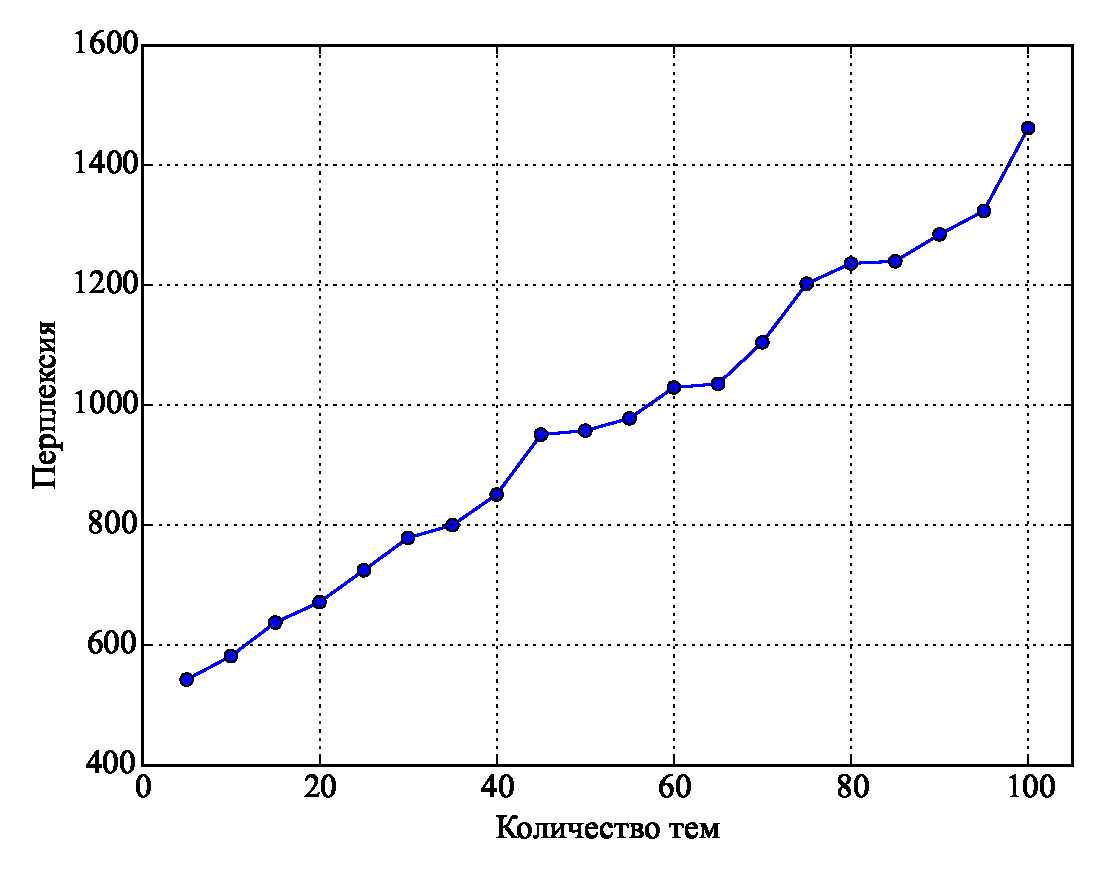
\includegraphics[totalheight=10cm]{perplexity_exp2}
    \caption{Изменение перплексии в зависимости от количества тем в программе Gensim}
    \label{fig:perplexity_gensim}
\end{figure}

Как видно из графика, в нашем случаем по мере увеличения количества тем перплексия также увеличивается, в то время как должен происходить обратный процесс -- большее количество тем лучше описывает распределение. Скорее всего это недостатки реализации расчёта перплексии в Gensim, поскольку сам автор программы признаёт наличие проблемы у некоторых пользователей\footnote{\href{https://groups.google.com/d/msg/gensim/TpuYRxhyIOc/JbTjqCcC6uYJ}{https://groups.google.com/d/msg/gensim/TpuYRxhyIOc/JbTjqCcC6uYJ}}.

Попробуем рассчитать перплексию с помощью другого инструмента и используем для этого популярную программу для тематического моделирования Mallet\footnote{\href{http://mallet.cs.umass.edu}{http://mallet.cs.umass.edu}}. Как упоминалось ранее, данная программа использует совершенно другой подход к тематическому моделированию, поэтому график \ref{fig:perplexity_mallet}, полученный в ней, сильно отличается от предыдущего. Как видно из графика, мы получили несколько локальных минимумов перплексии при 45, 60 и 85 темах.

\begin{figure}
	\centering
    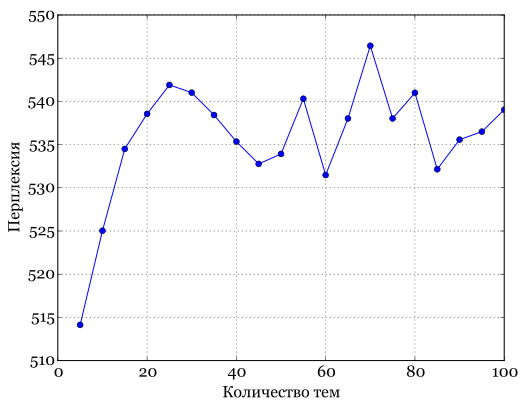
\includegraphics[totalheight=10cm]{perplexity_mallet}
    \caption{Изменение перплексии в зависимости от количества тем в программе Mallet}
    \label{fig:perplexity_mallet}
\end{figure}

Какие могут быль альтернативы расчёту перплексии? Во-первых, можно использовать алгоритмы тематического моделирования, которые автоматически подбирают оптимальное количество тем. Таким алгоритмом является, например, иерархический процесс Дирихле (hierarchical Dirichlet process, HDP), который напоминает LDA с то разницей, что данный подход относится к непараметрическим, а модель сама определяет оптимальное количество тем. Так как в Gensim присутствует реализация данного алгоритма, не составит труда применить его на нашей выборке.

В результате иерархического процесса Дирихле мы получили более 500 тем. Однако данное количество тем довольно сложно  интерпретировать, ведь нам необходимо проанализировать каждую тему и дать ей название.

Ещё один опробованный нами способ решения данной задачи описан в статье под названием <<О нахождении естественного числа тем в LDA: некоторые наблюдения>> \cite{Arun_KL}. В ней автор предлагает использовать  расстояние Кульбака — Лейблера как способ оценки качества модели. Чем меньше указанное расстояние, тем лучше модель. В результате расчёта этого расстояния на моделях с разным количеством тем, построенных в Gensim, мы получили график, показанный на рисунке \ref{fig:kl_div}.

\begin{figure}
	\centering
    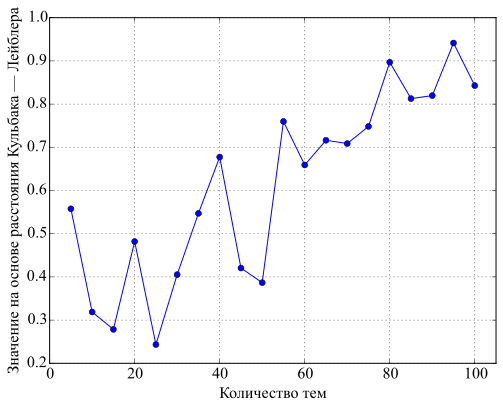
\includegraphics[totalheight=10cm]{kl_div}
    \caption{Изменение расстояния Кульбака — Лейблера в зависимости от количества тем в программе}
    \label{fig:kl_div}
\end{figure}

Из него видно, что оптимальное количество тем равняется 15, 25, 50.

В конечном итоге после сравнения моделей с разным количеством тем, мы выбрали модель с 50-ю темами, поскольку сгенерированные ей темы легче всего подвергались интерпретации и сильнее всего отличались друг от друга.

Полученные темы и их интерпретация представлены в приложении \ref{app:topics}. Как видно, в омских Интернет-СМИ представлен широкий спектр тем: от достаточно частных, касающихся ареста бывшего вице-мэра Юрия Гамбурга или убийства боксёра Ивана Климова, до взаимоотношений с Украиной и США.

Название темы определялись после анализа слов, которые эта тема генерирует с наибольшей вероятностью. Ниже показано, как программа описывает одну из тем. Рядом к каждым словом указана вероятность, с которой оно генерируется данной темой. Из этого распределения становится понятно, что данная тема имеет отношение к прогнозу погоды в городе Омске. Однако, как мы увидим позже, не все темы можно так легко интерпретировать.

\texttt{0.030*омск + 0.018*температура + 0.017*день + 0.015*снег + 0.014*погода + 0.014*воздух + 0.012*градус + 0.011*ветер + 0.010*область + 0.010*днём + 0.009*ожидаться + 0.009*дождь + 0.008*ночью + 0.007*выходной + 0.006*составить + 0.006*неделя + 0.006*управление + 0.006*м/с + 0.005*атмосферный + 0.005*тёплый}

Также мы можем рассчитать вероятностное тематическое распределение для каждого отдельного документа, выявив наиболее связанные с ним темы. Так как в LDA используется нечёткая кластеризация, каждый документ с определённой вероятностью можно отнести к любой теме. В связи с этим необходимо определить порог, который будет служить ориентиром для отнесения документа к каким-либо темам.

Здесь мы обнаруживаем, что при пороге в 0.1 один документ в среднем можно отнести к 6.64 темам, при пороге в 0.1 -- к 2.76. При пороге в 0.2 575 документов нельзя отнести ни к одной из тем.
\todo[inline]{И что это значит?}
% Для 0.1 (2.76 среднее): 3: 11250, 2: 10010, 4: 6519, 1: 4249, 5: 1652, 6: 194, 7: 3
% Для 0.01 (6.64 среднее): 6: 4988, 5: 4596, 7: 4373, 8: 3703, 4: 3655, 9: 2906, 3: 2669, 10: 1969, 2: 1396, 11: 1232, 12: 867, 13: 489, 1: 386, 14: 275, 15: 181, 16: 90, 17: 44, 18: 32, 19: 13, 20: 8, 21: 4, 23: 1

Итак, о чём пишут в омских Интернет-СМИ? Для ответа на этот вопрос, надо определить критерий, на основании которого среди множества тем, будет выбрана та, которая будет считаться основной для данного документа или множества документов. Самый просто способ -- отнесение документа к теме, в которую он попадает с наибольшей вероятностью. Таким образом мы получим, что самая популярная тема, которая наиболее вероятная для 1855 документов -- это ДТП (тема № 19), вторая по популярности, к которой относятся 1845 документов -- преступления (тема №43), третья (1609 документов) -- взаимоотношения с Украиной (тема №39). 

Этот способ хорошо подходит для определения темы отдельного документа, но если мы хотим таким способом оценить тематическое распределение на некотором множестве документов, то мы упустим важное преимущество LDA -- нечёткую кластеризацию, а именно возможность отнесения документа сразу к нескольким темам. Поэтому для выявления наиболее популярной темы во множестве документов разумно рассчитать среднюю вероятность для каждой темы путём сложения вероятностей всех тем для всех документов этого множества и деления на количество документов множества. В таком случае самыми популярными у нас будут темы под номерами 19 (ДТП), 43 (преступления) и 4 (пожары). Этот способ мы считаем предпочтительным. Полные результаты представлены в таблице \ref{table:popular_topics_2} приложения \ref{app:popular_topics}

Ещё один способ решения задачи поиска наиболее популярной темы во множестве документов -- объединение текстов данных документов и поиск вероятностного распределения для нового большого текста. При таком подходе на первый план вышли темы 2 (сложно интерпретировать), 39 (Украина), 1 (региональная власть).

Здесь мы встречаемся с такой проблемой, как сложность интерпретации некоторых выделенных тем. В нашем случае таких тем {написать количество}, а одна из них -- та самая тема номер 2 -- к тому же очень распространена. Проанализировав слова, которые она генерирует мы видим, что в них сложно найти что-то общее:

\texttt{0.009*человек + 0.007*большой + 0.006*нужно + 0.005*город + 0.005*омск + 0.005*время + 0.005*деньги + 0.005*сделать + 0.004*хороший + 0.004*вопрос + 0.004*делать + 0.004*знать + 0.004*проблема + 0.004*журналист + 0.004*работа + 0.004*работать + 0.004*должный + 0.003*проект + 0.003*метро + 0.003*думать}

К тому же вероятности, которыми тема генерирует данные слова чрезвычайно низки. Самая большая вероятность находится на уровне 0.009, в то время как в других темах примерно от 0.2 до 0.6

Одна из причин этому -- большое количество слов, которые ничего не могут сказать нам об особенностях темы. В основном это прилагательные и глаголы, которые обозначают признак предмета или его действие, но не называют сам предмет (большой, нужно, сделать, хороший и др.). Возможно, часть этих слов стоило занести в список стоп-слов.

Анализ документов, в которых проявление этой темы наиболее вероятно, также показывает сложность её интерпретации. Вот примеры заголовков некоторых из этих документов: <<Обзор блогов. Блоги – это маленькая жизнь>>, <<Сколько ещё простоят хрущевки в России?>>, <<Обзор СМИ: Страшно далеки они от народа>>, <<Кустурица стоя аплодировал омским рокерам>>.

Наличие таких <<мусорных>> тем -- нормальное явление в тематическом моделировании, которого тем не менее надо старательно избегать, проводя качественный препроцессинг документов и выбирая оптимальное количество тем для модели. В нашем случае сложности возникли с двумя темами, что можно считать неплохим результатом.

\section{Анализ комментариев}
\subsection{Общая характеристика}
Переходя к комментариям, мы вначале дадим общую их характеристику в данном корпусе. К 26783 статьям  из 33877 пользователи оставили 258121 комментариев -- это примерно 7.6 комментария на статью.

Относительно распределение комментариев во времени, можно сказать, что оно ожидаемо практически полностью повторяет распределение статей. Подробнее на рисунке \ref{fig:comments_by_day} приложения \ref{app:comments}.

\subsection{Комментируемость тем}
Определим самые резонансные темы, подсчитав, статьи какой тематики комментируют чаще всего, а какой -- реже. Для этого отнесём каждый документ к одной из тем, на основании  того, к какой теме он относится с наибольшей вероятностью. Затем рассчитаем отношение общего числа комментариев к статьям данной тематики к количеству этих статей. Полученное число и будет являться индикатором резонансности темы.
%[(25, 14.741982507288629), (39, 14.501243781094526), (13, 14.20414201183432), (36, 11.93984962406015), (48, 11.939705882352941), (2, 11.666666666666666), (27, 11.325714285714286), (22, 10.213058419243985), (47, 10.068592057761732), (32, 10.017227877838684), (35, 9.255172413793103), (23, 9.243027888446216), (37, 8.551063829787234), (11, 8.464699683877766), (41, 8.425096030729833), (21, 8.338530066815144), (1, 8.231625835189309), (16, 8.129562043795621), (24, 7.808035714285714), (5, 7.713768115942029), (9, 7.713603818615752), (19, 7.656418554476807), (17, 7.437858508604206), (34, 7.281399046104928), (42, 7.275862068965517), (0, 7.2066831683168315), (15, 7.127686472819216), (40, 6.427722772277228), (43, 6.4), (30, 6.347682119205298), (31, 6.001904761904762), (14, 6.0), (29, 5.90400604686319), (7, 5.847154471544715), (6, 5.493201483312732), (10, 5.476054324517513), (44, 5.266528925619835), (12, 5.248339973439575), (46, 5.246478873239437), (45, 5.137835337650324), (3, 4.810490693739425), (38, 4.743935309973046), (26, 4.7139917695473255), (4, 4.537396121883656), (33, 4.429467084639499), (20, 4.331550802139038), (49, 4.243523316062176), (28, 4.058997050147493), (8, 2.722408026755853), (18, 1.5898123324396782)]

Как и в случае с расчётом наиболее популярной темы, помня что каждый документ можно отнести ко многим темам,  в эту формулу можно внести улучшения. Более валидные результаты мы получим, рассчитывая показатель комментируемости темы путём сложения рассчитанных для каждого документа произведений вероятности присутствия темы в документе на количество комментариев в данном документе. Таким образом, по итогам наших вычислений было выявлено, что самыми комментируемыми темам являются темы 39 (Украина), 25 (Домашние животные), 13 (Арест Юрия Гамбурга). Причём интересно, что тема, связанная с событиями на Украине, почти вполовину обгоняют ближайшую конкурирующую тему.


% [(39, 17244.5922226523), (19, 12490.240793933619), (32, 11586.258992149169), (2, 11370.18542959649), (1, 11012.687969142713), (43, 10083.558099992124), (25, 10006.136640068615), (11, 8824.876084640866), (36, 8697.518177116868), (16, 7864.1535496519155), (48, 7511.644975212715), (10, 7238.399488896429), (15, 6893.099994404986), (7, 6701.672949136045), (29, 6496.275602983442), (4, 6280.852746070645), (0, 6045.058109970468), (41, 5635.074475729932), (6, 4948.64015425139), (5, 4546.114921615737), (13, 4368.2005320091475), (37, 4352.295105311304), (45, 4338.78434455233), (12, 4253.452439532452), (21, 4056.7049351304267), (17, 3834.5084463028516), (34, 3598.043918354743), (22, 3596.710092384489), (9, 3572.0507135379858), (3, 3498.9689308144734), (40, 3302.7595825734024), (20, 3097.207627469377), (31, 3082.189339025612), (47, 3056.177635745364), (23, 3017.2008352042762), (26, 2877.665839985531), (44, 2384.9391681981174), (38, 2383.5193405682458), (24, 2357.371627628458), (42, 2190.402604832842), (30, 2089.9195411730234), (33, 2070.0522347395195), (27, 2027.1834046991003), (28, 1830.4461533787617), (49, 1821.9336546257912), (8, 1767.0680351472013), (35, 1634.6784882912968), (46, 1603.3388512369452), (14, 962.5362328876633), (18, 890.8390328596042)]

% Есть умножить на популярность темы, будет
% [(39, 466794.4839104599), (25, 438587.41828490666), (13, 405364.2262510703), (36, 373075.0501371295), (2, 355910.23290679615), (48, 349523.98583821027), (22, 328142.3515352057), (27, 325262.4470055852), (47, 314311.9240306591), (32, 306476.511632714), (14, 303975.52692883083), (37, 303645.9904334151), (11, 288482.15107184584), (1, 287409.3612508797), (23, 284725.52456481213), (16, 274584.23424592725), (21, 273964.63247706136), (15, 270394.3898096543), (41, 268870.697295894), (42, 266407.3012991383), (35, 261548.1279847216), (19, 261130.34107368896), (9, 254836.17015757255), (5, 253670.7192758214), (24, 252749.70389157426), (0, 240659.3037026888), (17, 237992.40131337958), (34, 229088.19468558038), (43, 225123.02891694114), (46, 223780.96737727348), (40, 216745.03542798522), (31, 215439.53275631834), (7, 214176.14245982532), (6, 209028.96520340495), (10, 208889.61842837682), (30, 202085.01028213426), (3, 198766.56231538582), (29, 194878.62567135828), (33, 192648.85439201046), (12, 187617.60598127465), (38, 185746.93615677548), (44, 184636.81631191837), (26, 182812.414188796), (45, 180474.7808397816), (20, 172897.52215932752), (28, 172639.3951259277), (49, 165307.5922918495), (4, 161619.03964644053), (8, 159437.4754193113), (18, 96475.34663398893)]

\subsection{Анализ тональности комментариев}
Анализ тональности -- ещё одна сфера интеллектуального анализа текста. Да данном этапе мы собираемся оценить тональность комментариев к различным темам. Гипотеза заключается в том, что если существует какая-то социальная напряжённость в обществе по отношению к какой-либо теме, то это находит выражение в комментариях к статьям соответствующей тематики. Наша задача, таким образом, состоит в том, чтобы найти темы, которые вызывают социальную напряжённость.

Существует несколько подходов к классификации тональности. Первый подход основан на наборе правил, применяя которые система делает заключение о тональности текста. Например, для предложения «Я люблю кофе», можно применить следующее правило: если сказуемое (<<люблю>>) входит в положительный набор глаголов (<<люблю>>, <<обожаю>>, <<одобряю>> ...) и в предложении не имеется отрицаний, то классифицировать тональность как <<положительная>>. Многие коммерческие системы используют данный подход, несмотря на то что он требует больших затрат, т.к. для хорошей работы системы необходимо составить большое количество правил. Зачастую правила привязаны к текстам определённой тематики (например, «ресторанная тематика») и при смене тематики («обзор фотоаппаратов») требуется заново составлять правила. Тем не менее, этот подход является наиболее точным при наличии хорошей базы правил.

Следующий подход основан на машинном обучении, чаще всего с учителем. В этом случае необходимо разметить некоторое количество текстов, на которых обучается подстроенная с помощью каких-либо алгоритмов модель. Часто для этого используется обычный байесовский классификатор. В дальнейшем эта модель распределяет тексты по заданным категориям. Это достаточно простой метод, а потому он широко распространён. Недостатками метода является невысокая точность ($\approx70$\%) и необходимость ручной разметки обучающей выборки.

Подходы, основанные на словарях, используют так называемые тональные словари (affective lexicons) для анализа текста. В простом виде тональный словарь представляет из себя список слов со значением тональности для каждого слова. Каждому слову из словаря, встречающемуся в тексте присваивается соответствующее значение, а затем вычисляется общая тональность текста.

Существует не так много бесплатных программ, предназначенных для анализа тональности текста. Ещё меньше из них -- а в действительности ни одна из них -- умеют адекватно определять тональность текстов на русском языке. В таких сложных условиях наилучшим вариантом нам виделась программа SentiStrength\footnote{\href{http://sentistrength.wlv.ac.uk/ }{http://sentistrength.wlv.ac.uk/}} за авторством Майкла Фелвола\footnote{Глава Statistical Cybermetrics Research Group университета Вулверэмптона, ассоциированный научный сотрудник Oxford Internet Institute, Великобритания.}. Будучи бесплатной для некоммерческого использования, данная программа может работать почти с любым языком и, по крайней мере со стандартными словарями для английского языка, показывает хорошие результаты \cite{SentiStrength}. Для работы с другими языками, необходимо загрузить в неё тональные словари на нужных языках. Основания часть этих словарей представляют собой простой текстовый файл со списком слов, к каждому из которых в поставлена в соответствие оценка позитивной (по шкале от 1 до 5) или негативной составляющей (по шкале от -1 до -5). Большее значение соответствует большей выраженности эмоциональной составляющей. Другие части словаря, также представляющей собой текстовые файлы, содержат список слов-усилителей, которые усиливают значение тональности для слова, на которое они действуют (<<очень плохой>> будет иметь более негативную оценку, чем просто <<плохой>>), идиоматические выражения, слова-отрицания, смайлы, вопросительные слова, сленговые слова и слова обозначающие иронию. Все эти части учитываются алгоритмом и помогают достичь более точного результата. Результат выдаётся в виде двух оценок – оценка позитивной составляющей текста (по шкале от +1 до +5) и оценка негативной составляющей (по шкале от -1 до -5) или в виде бинарной оценки (позитивный/негативный текст).

Но в этих словарях и кроются самые большие сложности использования программы. Первая версия словарей для русского языка\footnote{\href{http://sentistrength.wlv.ac.uk/SentStrength\_Data/russian}{http://sentistrength.wlv.ac.uk/SentStrength\_Data/russian}}, созданная факультетом прикладной лингвистики Санкт-Петербургского государственного университета аэрокосмического приборостроения, не отличается хорошим качеством. Из-за излишне общих правил данные словари часто оценивали нейтральные слова как эмоционально окрашенные\footnote{Дело в том, что в словарях к SentiStrength для создания простых правил можно использовать оператор *, который обозначает любое количество любых символов кроме пробела. Под шаблон <<*плом*>>, например, подходят слова <<\textbf{плом}ба>>, <<ди\textbf{плом}ированный>> и др. В своих словарях авторы переусердствовали с применением данного оператора. Это привело, например, к тому, что словари дают три балла негативной эмоциональной составляющей любому слову, начинающемуся на <<ад>> (приравнивая \textbf{ад}министраторов к исчадиям \textbf{ад}а) и два балла позитивной словам на <<мил>> (а это далеко не только слово <<\textbf{мил}ый>>, как вероятно задумывали авторы словарей, но вызывающее не самые позитивные эмоции слово <<\textbf{мил}иция>>).}.

Вероятно, по этой причине для своего исследования тональности комментариев к постам в Живом Журнале, коллективом Лаборатории Интернет-Исследований был создан новый тональный словарь\footnote{\href{http://sentistrength.wlv.ac.uk/SentStrength\_Data/russian2}{http://sentistrength.wlv.ac.uk/SentStrength\_Data/russian2}}\cite{hse_sentistrength}. Процесс адаптации включал в себя перевод англоязычного словаря, на основе которого работает ПО, на русский язык, подбор подходящих русских эквивалентов к полученным словам, составление частотного словаря на основе комментариев к постам ЖЖ, включение частотных слов в словарь и кодирование словаря по шкале эмоциональности от -5 до 5. После проверки результатов работы программы с результатами ручного кодирования был сделан вывод, что количество совпадений между автоматическим кодированием с данным словарём и ручным значительно уступает аналогичным экспериментам на английском языке.

По сравнению с первым вариантом словаря, второй вариант обладал прямо противоположной проблемой -- тенденция оценивать негативно эмоционально окрашенные тексты как нейтральные\footnotemark \cite[стр. 3]{hse_sentistrength}. 

\footnotetext{
		Нами было выделено несколько вероятных причин проблем у второго варианта словаря. Главная из них заключается в том, что словарь состоит только из слов в нормальной форме и оператор * в них не используется. Поэтому для оценки текстов с использованием этого словаря необходима предварительная лемматизация. Сотрудники Лаборатории Интернет-исследований, естественно, знали об особенностях своих словарей и не обошли вниманием этот этап.
		
		Здесь, однако, стоит сказать, что лемматизация достаточно плохо работает на словах, которые ярче всего свидетельствуют о негативных эмоциях -- обсценной лексике. Для лемматизации необходим словарь со всеми словоформами, но мат в эти словари включают редко.
		
		К тому же, многие программы, производящие лемматизацию (тот же используемый нами pymorphy2), при приведении слова к нормальной форме не отбрасывают при этом приставки (<<набрал>> $\rightarrow$ <<набрать>>, а не <<брать>>), которые играют огромную роль в обсценной лексике. В такой ситуации необходимо включать в словарь слова обсценной лексики со всеми вариантами приставок, что сложно при наличии проблемы, указанной в предыдущем абзаце.

		Ещё одна возможна причина неудовлетворительного результата работы второго варианта словаря может заключаться в том, что для перед лемматизацией  необходима токенизация. Но SentiStrength предназначена для анализа <<сырого>> текста сама производит токенизацию по своему специфическому алгоритму. Так конструкция <<какое-либо-слово)))>> благодаря тому, что смайл и слово являются одним целым, будет присвоено два балла положительного эмоционального заряда. Но если отделить смайл от слова <<какое-либо-слово )))>>, то программа просто не увидит здесь никакой эмоции.

		Возможно, лучший результат дала бы замена лемматизации на стемминг. Так как для стемминга не нужна база основ слов, а лишь правила и набор морфем, проблема обсценных слов была бы решена.
}

%На сайте SentiStrength был найден ещё один словарь, происхождение которого нам неизвестно \footnote{\href{http://sentistrength.wlv.ac.uk/SentStrength\_Data/russian/Russian\%20May\%202011.zip}{http://sentistrength.wlv.ac.uk/SentStrength\_Data/russian/Russian May 2011.zip}}. В нём не использовался оператор *, но словарная база превосходила по объёму второй вариант словаря. Впрочем, не все слова из этого словаря были адекватно оценены (аргумент -2, аккумуляторов -2). Вероятно, данный словарь создавался для оценки текстов специфической тематики, и там такая оценка тональности была корректна, но в нашем случае лучше будет избавиться от неё.

Общим недостатком рассматриваемых русскоязычных словарей является практически полное отсутствие в них идиоматических выражений, сленговых и ироничных слов.

В условиях невысокого качества словарей, было принято решение о создании нового тонального словаря. В целях экономии ресурсов было решено построить его на основе предыдущих версий, учтя их достоинства и недостатки, с добавлением специфичных для исследуемых текстов эмоционально окрашенных слов.

Основой для построения нового словаря стал первый словарь. Главная проблема данного словаря -- слишком нестрогие правила, допускающее большое количество ложных соответствий.

Первым делом из него были удалены правила, касающиеся слов меньше, чем из четырёх символов и допускающие некорректные соответствие словам (правило ад* допускало соответствие слову администратор). Правила были преобразованы в обычные слова (ад). Затем все слова (только слова, не правила) с помощью программы pymorphy2, были развёрнуты в различные свои словоформы (ад, ада, адом и др.) Таким образом явное указание подходящих слов позволило уйти от лишком общих правил.

Второй словарь, который, напомним, состоял только из нормальных форм и требовал лемматизации поступающих слов, было решено преобразовать к формату первого. Для этого слова данного словаря длинной больше трёх символов были пропущены через процедуру стемминга, с последующей заменой усечённых частей на оператор *. Для более коротких слов, как и в предыдущем случае, были найдены все словоформы.

Затем получившиеся словари были объединены и в получившийся список были добавлены 113 тональных слов, выделенных на основании изучения более двухсот случайных комментариев из исследуемой выборки и отсутствующих в исходных словарях. Баллы данным словам выставлялись на основе произвольного мнения автора, что нельзя признать методологически корректным. Однако это лучше, чем ничего.

Конструирование нового словаря закончилось удалением повторяющихся записей.

Новый словарь обладает следующими преимуществами:

\begin{enumerate}
\item Он объединяет словарные базы двух разных словарей, а значит полнее их.
\item Для пользования данным словарём не надо модифицировать входящие данные.
\item Данный словарь включает слова, которых не было ни в одном из предыдущих. Некоторые их этих слов специфичны для исследуемых текстов (например, слово <<укроп>>)
\item Правила нового словаря корректнее, точнее, чем правила первого словаря, а значит ложных срабатываний будет меньше.
\end{enumerate}

\clearpage